\section{Saját módszer} \label{sec:new_method}

Ebben a részben részletezzünk az általunk implementált módszert. A cél egy olyan rendszer felépítése, amely a már meglévő statisztikus gépi fordítás rendszereket egészíti ki egy jelentés egyértelműsítést szolgáltató (WSD) rendszerrel. Az SMT rendszerek gyakran rossz eredményt adnak abban az esetben, amennyiben a fordítandó szavak több jelentéssel is bírnak. Ezekben az esetekben nyújthat segítséget egy ilyen bővítmény, amely képes a szövegkörnyezet alapján meghatározni a szó tényleges jelentését, és így egy pontos fordítást adni az adott mondatra. 

Tárgyaljuk a felhasznált Wikipedia alapú WSD modult, valamint részletezzük annak alkalmazását egy meglévő SMT rendszerben.

\subsection{Wikipedia alapú jelentés egyértelműsítés} \label{sec:WikiWSD}

Egy korábbi munkában \cite{gabrilovich2007computing} bevezettek egy Wikipedia oldalakon alapuló módszert, amelyben a cikkek címeit mint fogalmakat tekintették, amelyeket egy adott szó jelentésének leírására használták fel. A Wikipedia esetünkben is egy jó megoldásnak bizonyult, hiszen a világ egyik legnagyobb nyílt enciklopédiája (az angol változat több, mint 400 millió szót és több, mint 1 millió cikket tartalmaz), a tartalom különböző cikkekbe van rendezve, és ami a számunkra legfontosabb, hogy ugyanazok a cikkek több nyelven is elérhetőek, és ezek között a cikkek között egy jól meghatározott megfeleltetés is van. Ezekből az okokból kifolyólag mi is egy hasonló rendszer alkalmazása mellett döntöttünk.

A cél egy szemantikus értelmező építése, amely képes egy szóhoz vagy egy szövegrészlethez egy súlyozott fogalomvektort hozzárendelni. A vektor elemei az adott szövegrészlethez kapcsolódó fogalmak lesznek, míg a súlyok azt határozzák meg, hogy mennyire jellemző az adott fogalom a szövegre. Amikor fogalmakról beszélünk továbbra is a cikkek címét értjük. 

Minden Wikipedia cikket egy attribútum vektorként reprezentálhatunk. A vektor minden eleme megadja, hogy az elemhez tartozó szó mennyire releváns a cikk címe által reprezentált fogalomra. A relevanciát a szóhoz tartozó TFIDF súllyal fejezzük ki. Jelölje $k_t$ az $t$ szóhoz tartozó TFIDF súlyt. Ekkor 
\begin{equation}
	k_t = \frac{tf_t}{df_t}
\end{equation}
ahol $tf_t$ a $t$ szó előfordulásainak a száma a cikkben, míg $df_t$ azoknak a dokumentumoknak a száma, amelyben $t$ előfordul.

Ahhoz, hogy a szemantikus értelmezést gyorsabban el tudjuk végezni, egy invertált indexet építünk fel, vagyis minden szóhoz egy fogalomlistát rendelünk, amelynek mindegyik eleme az adott fogalom és a szó TFIDF súlya az adott fogalomhoz tartozó cikk esetében. Ezen kivül, hogy a felhasznált tárhelyet megfelelően alacsonyan tudjuk tartani, csak azokat a fogalmakat őrizzük meg ebben a listában, ahol a hozzárendelt súly átlép egy küszöbértéket (\ref{fig:invindex}. ábra).

\begin{figure}[ht]
	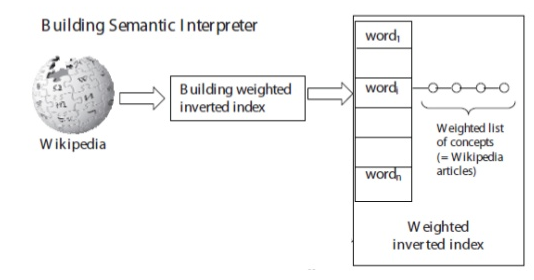
\includegraphics[scale=0.3]{images/invindex} 
	\caption{Invertált index}
	\label{fig:invindex}
\end{figure}		

Mivel a fordítás során a bemeneti szövegek nyelve különböző, fel kell építenünk egy invertált indexet minden nyelvhez, amit használni szeretnénk. Ehhez fontos az is, hogy legyen egy megfeleltetésünk a különböző nyelvű cikkek és ezáltal fogalmak között, ezt azonban a Wikipedia felépítése direkt módon megadja.

Két szöveg összehasonlításához szükséges, hogy az egyes szövegekhez hozzá tudjunk rendelni egy fogalomvektort. Jelölje $T = \{w_i\}$ a bemeneti szöveget, ahol $w_i$ egy szó. Minden $w_i$ szóhoz társítsuk a $v_i$ TFIDF súlyt, ahol a $tf_i$ tagot ezúttal a szó előfordulásainak számát jelenti a bemeneti szövegben. Minden szóhoz társítsunk egy $k_{i,j}$ elemekből álló vektort, ahol egy elem az $w_i$ szó $c_j$ fogalmomhoz tartozó súlyát jelenti az invertált index alapján. A teljes szöveg súlyvektorának $j.$ komponensét ekkor a 
\begin{equation}
\sum_{w_i \in T} v_i \cdot k_{i,j}
\end{equation}
adja (\ref{fig:textfragment}. ábra)

\begin{figure}[ht]
	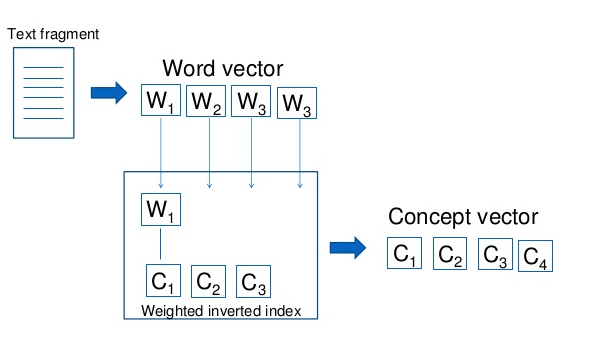
\includegraphics[scale=0.3]{images/textfragment}
	\caption{Fogalomvektor felépítése bemeneti szöveg alapján}
	\label{fig:textfragment}
\end{figure}	

Az előbb leírt módon előállított súlyvektorokat felhasználva a két vektor koszinusz távolságának kiszámolásával megadhatjuk a két szöveg szemantikai hasonlóságát (\ref{fig:similarity}. ábra). Legyen $\overrightarrow{u}$ és $\overrightarrow{v}$ a két súlyvektor, ekkor a két szöveg hasonlósága: 
\begin{equation}
	sim_{u,v} = \frac{\overrightarrow{u} \cdot \overrightarrow{v}}{\left\lVert \overrightarrow{u} \right\rVert \cdot \left\lVert \overrightarrow{v} \right\rVert}
\end{equation}

\begin{figure}[ht]
	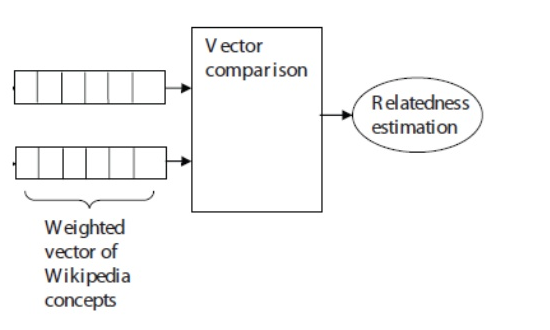
\includegraphics[scale=0.3]{images/similarity}
	\caption{Hasonlóság meghatározása súlyvektorokból}
	\label{fig:similarity}
\end{figure}	

\subsection{WSD modul beépítése SMT rendszerbe} \label{sec:WSDinSMT}

Az egyik legegyszerűbb és jól működő modell a jelentés egyértelműsítés SMT rendszerekbe való integrációjára az $n$ legjobb elem újrarangsorolása (\cite{apidianaki2012wsd}).

Első lépésként felhasználjuk a standard SMT rendszerünket, amely segítségével kapunk $n$ darab lehetséges fordítást a bemeneti szövegre. Az így kapott fordításokat és a bemeneti szöveget felhasználva a \ref{sec:WikiWSD}. részben tárgyalt módszer segítségével minden fordításhoz hozzárendelhetünk egy súlyt. Az SMT által és a WSD által adott súlyokat is normalizáljuk, majd ezeket összeadjuk. A végső fordítás az így kapott súlyok szerinti legjobb eredmény lesz:

\begin{equation}
	f = argmax_i (\frac{w_{SMT, i}}{\left\lVert w_{SMT} \right\rVert} + \frac{w_{WSD, i}}{\left\lVert w_{WSD} \right\rVert})
\end{equation}